

In~\cref{ssec:layout} we present \sys's data organization. 
We discuss concurrency control and atomic scans in~\cref{ssec:scans}.
\cref{ssec:ops} overviews \sys's normal %(maintenance-free) 
operation flow, while   the data structure's maintenance is discussed in~\cref{ssec:rebalance}.
Finally,~\cref{ssec:flush-recovery} discusses data flushes and failure recovery.


\subsection{Data organization}
\label{ssec:layout}

% \paragraph{Chunks, funks, and munks.}

\sys's data layout is depicted in Figure~\ref{fig:piwi}.
Data is partitioned into chunks, each holding a contiguous key range.
Each chunk's data 
(keys in its range and their corresponding values) 
is kept on-disk (funks, for persistence), and possibly in-memory (munks, for fast access). 
Munks can be replaced and loaded from funks at any time based on an arbitrary replacement policy.
Chunk metadata objects are significantly smaller than munks and funks
(typically, less than 1 KB vs. tens of MBs) and are always kept in memory.

A volatile \emph{index} maps keys to chunks. 
Index updates are lazy, offering only best-effort expedited search.

A funk consists of two files:  a compacted and sorted KV map \emph{SSTable} %(Sorted String Table~\cite{Bigtable2008}) 
and a write \emph{log}. When a funk is created, the {former} holds all the chunk's KV pairs and the {latter}  is empty.
New KV pairs are subsequently appended to the  {log}. If a key is over-written, its old value remains in the {SSTable} while the new one  is added to the {log} (the {log} is more up-to-date).

\remove{
\begin{figure}[tb]
\centerline{
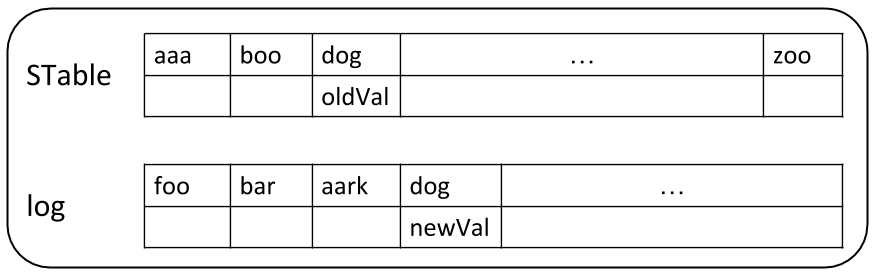
\includegraphics[width=0.75\columnwidth]{funk.png}
}
\caption{A \sys\ funk consists of a sorted {SSTable} and an unsorted {log} holding the most recent updates.}
\label{fig:funk}
\end{figure}
}

This structure allows us to benefit from sorted searches on the {SSTable} and at the same time
to update chunks without relocating existing data, thus minimizing write amplification.
As a funk's {log}  grows, however, searching becomes inefficient   and  
the funk is no longer compact, i.e., it may contain redundant (over-written) values.
Therefore, once the {log}  exceeds a certain threshold, we reorganize the funk
via a process we call \emph{rebalance}, as explained below.

% Thus, multiple \emph{generations} of munks may exist for a chunk throughout its life time.
%Chunks that are not cached are denoted \emph{munk-less}.
%The details of the chunk's metadata structure are deferred to the the supplemental material.

A munk holds KV pairs in an array-based linked list.  
\remove{
A munk consists of two arrays -- \emph{karray} for keys and \emph{varray} for values. The  \code{karray}  holds a sorted linked list of the chunk's keys
with pointers to values in the \code{varray}. 
}
When a munk is created, some prefix of this array is populated,
sorted by key, so each cell's successor in the linked list is the ensuing cell in the array.
New KV entries are appended after this prefix.
As new entries are added, they create bypasses in the linked list, and consecutive keys in the
list are no longer necessarily adjacent in the array. Nevertheless, as long as 
a sizable prefix of the  array  is sorted and insertion order is random, bypasses are short in expectation.
\remove{Key removals, in turn, leave obsolete values in the munk, so it is no longer compacted.}
Keys can thus be searched efficiently via binary search on the sorted prefix followed by a short traversal 
of a bypass path. % at the suffix of the array. 
%This approach was previously used in in-memory data structures, e.g., Kiwi~\cite{kiwi}.  

As KV pairs are added, overwritten, and removed, munks and funks need to undergo reorganization. This includes  
(1) \emph{compaction} to garbage-collect removed and overwritten data, 
(2) \emph{sorting} keys to make searches more efficient,  and
(3) \emph{splitting} overflowing chunks.
Reorganization is performed by three procedures: 
(1) Munk rebalance (creating a new compacted and sorted munk instead of an existing one) 
happens in-memory, independently of disk flushes. 
(2) Funk rebalance (on-disk) happens much less frequently. 
(3) Splits  create new chunks as well as new  funks and munks.

%\paragraph{Expediting reads.}

Whenever a chunk is cached (i.e., has a munk), access to this chunk is particularly fast:
the chunk metadata is quickly located using the index, the munk's sorted prefix allows for fast 
binary search, and updates are added at the end of the munk's array and appended to the funk's log.
% Thus, \sys\ is particularly fast when almost the entire working set is memory-resident. 
We take two measures to mitigate the performance penalty of accessing keys in non-cached chunks.

First, we keep a row cache holding popular KV pairs only from munk-less chunks. Note that unlike munks, which cache key ranges, the row
cache holds individual keys, and is thus more effective in dealing with point queries (gets as opposed to scans) with no
spatial locality.

If the active working set is larger than the available DRAM, these two caches might not suffice, and so a certain portion of reads 
will be served from disk. Here, the slowest step is the sequential search of the {log}. 
To reduce such searches, a chunk with no munk holds a Bloom filter for the corresponding funk's {log}, 
which eliminates most of the redundant log searches.
The Bloom filter is partitioned into a  handful of filters, each summarizing the 
content of part of the {log}, limiting  sequential  searches to a small section of the log.
 
 \subsection{Concurrency and atomic scans}
\label{ssec:scans}
 
\remove{
\paragraph{Chunk metadata structure.}

The metadata structure is given in Algorithm~\ref{alg:chunk}. 
The first field is its \code{state}, which is explained in \cref{ssec:rebalance}  below. 
It next holds a pointer to the appropriate funk, and either a munk or a Bloom filter, as well as a pointer to the next 
chunk in the chunk linked list.
\remove{
It further keeps the generation number of its latest munk, \code{gen}, and a per-generation sequence number,
\code{seq}, which, in case there is an active munk, is the index of the next free cell in the munk's  \code{karray}  and \code{varray}. The chunk's \code{gen} and \code{seq} are stored together in one 64-bit word to allow 
atomic access to both of them. 
}
%It further includes a Bloom filter as explained above.
Finally, the chunk includes locks to synchronize concurrent access by multiple threads, as explained below.

\begin{algorithm}[htb]

\begin{algorithmic}
\State \code{state} \Comment  baby, child, active, asleep, or aged
\State ptr \code{funk} \Comment funk disk address
\State ptr \code{munk} \Comment munk memory pointer
\State ptr \code{next} \Comment next chunk in linked list
%\State int \code{gen} \Comment munk generation
%\State int \code{seq} \Comment sequence number in current generation 
\State ptr \code{bloomFilter} \Comment summary of set of keys in \code{log}
\State asymmetric lock \code{rebalanceLock} \Comment shared/exclusive lock 
\State lock \code{funkChangeLock} \Comment acquired with try\_lock 
% \State \code{$\langle$key, version, done, counter$\rangle$  PPA[threads]} \Comment pending puts
\end{algorithmic}

\caption{Chunk metadata structure.}
\label{alg:chunk}
\end{algorithm}
}

%\paragraph{Thread synchronization variables.}

\sys\ allows arbitrary concurrency among operations. Gets are wait-free and proceed without synchronization. 
In order for scans to be atomic, they synchronize with puts, potentially waiting for some puts to complete
(puts never wait for scans). Puts also synchronize with rebalance operations. 
% (invoked in background threads). 

\remove{
We note that using a single pending array to synchronize all operations can cause contention, which we
eliminate in our implementation by tracking the pending puts in per-chunk arrays with per-thread entries as done in~\cite{kiwi}.
}

To support atomic scans we employ a system-wide \emph{global version (GV)}. 
A scan  creates a \emph{snapshot} associated with GV's current value by fetching and incrementing GV.
This signals to ensuing put operations that they must not overwrite the highest
version smaller than the new GV value.
This resembles a \emph{copy-on-write} approach, which  creates a virtual snapshot by 
indicating that data pertaining to the snapshot should not be overwritten in-place.  

To allow garbage collection of old versions, \sys\  tracks the snapshot times of active scans.
This is done in a dedicated  \emph{Pending Operations (PO)} array, which has one entry per active thread,
and is also used to synchronize puts with scans as explained shortly.
The compaction process 
%that runs as part of rebalance 
removes old versions that are no longer required for any  
scan listed in PO. Specifically, for each key, it removes versions older than the highest version smaller than the minimal
scan entry in PO and the value of GV when the rebalance begins. 

\remove{
For linearizing (i.e., determining an order on) updates, we associate each KV pair written to the data store 
with a unique-per-key timestamp.
This timestamp is composed as a tuple $\langle$ver, gen, seq$\rangle$, where \emph{ver} is  the version read from GV 
(recall that GV is only incremented upon scans and hence might remain unchanged across multiple puts),
\emph{gen} is the generation of the target chunk's last created munk  (which may or may not still exist), 
and seq is the running sequence number of values inserted to the chunk in the current generation.
}

% \paragraph{Concurrent puts and scans.}

A put obtains a version number from GV without incrementing it. Thus, multiple puts may write values with the same version, each over-writing the previous one. 
%Ordering concurrent puts with the same key and version is discussed in the next section where we elaborate on the put operation's logic.

%A scan begins by fetching-and-incrementing GV.
If a put obtains its version before a scan increments GV, the new value must be included in the scan's snapshot. 
However, because the put's access to the GV and the insertion of the new value to the chunk do not occur atomically,
a subtle race may arise. Assume a put obtains version $7$ from GV and then stalls before
inserting the value to the chunk while a scan obtains version $7$ and increments GV to $8$. If the scan proceeds 
to read the affected chunk, it misses the new value it should have included in its snapshot.
%
To remedy this, puts announce (in PO) the key they intend to change when beginning their operations and scans wait for relevant pending puts to complete; see the next section for details.
%This mechanism is a simplification of the non-blocking put-scan synchronization employed (and proven correct) in~\cite{kiwi}.

%For symmetry, get operations synchronize with puts the same way that scans do. 

\remove{
A put operation takes hold of the chunk's \code{rebalanceLock} in shared mode, 
then publishes itself in  PO, gets a version by reading GV, updates its version in PO,  
and releases the chunk lock. 
}


\remove{
% Simplified PPA
  The per-chunk PPA is used to synchronize pending puts  with ongoing scans. It holds an entry for every active inserting thread, consisting of a \code{key},  a \code{version}, 
 a \code{done} bit indicating whether the update has been completed, and a monotonically increasing 
 \code{counter} to avoid ABA scenarios.
 
A put operation first registers itself in the appropriate chunk's PPA entry with the key it intends to put.
It then reads GV and sets the version field in its PPA entry to the read version. 
After completing the actual put (in the appropriate munk and/or funk), it sets the \code{done} bit.
A scan, in turn, scans the PPA in addition to the chunk's data 
(\code{karray},  \code{log} or \code{SSTable}  ). If it finds a pending put
of a relevant key that is not yet associated with a version, it waits for the version to be assigned. 
Once the version is assigned, if it is the highest version for this key that does not exceed its scan time, 
it waits for the \code{done} bit to be true or for the the \code{version} to change again, at  which point
it reads the value from the appropriate munk or funk.
}

Rebalance operations synchronize with concurrent puts using the chunk's \emph{rebalanceLock}.
This is a shared/exclusive lock, acquired in shared mode by puts and in exclusive mode (for short time periods)
by rebalance. 
%, which is held for short time periods during chunk, funk, and munk replacements.  
Gets and scans do not acquire the lock. Note that it is safe for them to read from a chunk while it is being replaced because
(1) rebalance makes the new chunk accessible only after it is populated, and (2) a chunk is immutable during rebalance, so 
the newly created chunk holds the same content as the displaced one.

To minimize I/O, we allow at most one thread to rebalance a funk at a given time. This is controlled by 
the  \emph{funkChangeLock}, which is held by the thread rebuilding the  chunk. 
It is acquired using a try\_lock, where threads that fail to acquire it do not retry but instead wait for the winning thread to complete the funk's creation.

\subsection{\sys\ operations}
\label{ssec:ops}

\Cref{alg:ops}  presents pseudocode for \sys's operations. 
Both get and put begin by locating the target chunk using the \code{lookup} function. In principle, this can be done by traversing the chunk list, but that would result in linear search time. To expedite the search,   \code{lookup} first searches the index. But because index updates are lazy -- they occur after the new chunk is already
in the linked list --  the index may return a stale chunk that had already been replaced by rebalance. To this end, the index search is repeated with a smaller key in case the index returns a stale chunk, and the index search is supplemented by a linked-list traversal. 
%A similar approach was used in earlier works~\cite{kiwi,tdls}. 


\begin{algorithm}[tb]
\begin{algorithmic}[1]{}
\Procedure{get}{key}	
		\State $C \leftarrow$ \code{lookup(key)}

%		\State $T \leftarrow  \{ \langle \code{th}, i \rangle : \code{C.PPA[th].key = key }  $ 
%		\Statex \hspace{21mm}	$ \wedge \; \code{C.PPA[th].counter} = i \}$ 



%		\code{th} $\in T$,  
%		\Statex  \hspace{21mm}		$C.$\code{PPA[th].done} $\vee$ \code{$C$.PPA[th].ver $>$ gv}
		\If{$C$.\code{munk}} 
			\State search \code{key} in $C$.\code{munk} linked list;  return 
		\EndIf
		\State search \code{key} in row cache; return  if found
		\If{\code{key}$\in C.$\code{bloomFilter}}  
			\State	search \code{key} in \code{funk.log}; return  if found
		\EndIf
		\State	search \code{key} in \code{funk.SSTable}; return  if found
		\State return NULL	
\EndProcedure
\Statex
\Procedure{put}{key, val}	
		\State $C \leftarrow$ \code{lookup(key)}
		\State lockShared($C$.\code{rebalanceLock})
		\State  \code{PO[i]}  $\leftarrow$ \code{$\langle$put, key, $\bot \rangle$ }
			 \Comment publish  thread's presence 
		\State \code{gv} $\leftarrow$ \code{GV}   \Comment read global version
		\State  \code{PO[i]}  $\leftarrow$ \code{$\langle$put, key, gv$\rangle$ }
			\Comment write version in \code{PO}
%		\Statex \Comment atomically allocate entry in munk and get its pointer
%		\State \code{$\langle$gen, seq$\rangle$ } $\leftarrow$ F\&I ($C$.\code{$\langle$gen, seq$\rangle$})
%		\State \code{munk} $\leftarrow$ $C$.\code{munk} \Comment read atomically with \code{gen}
		\Statex \Comment write  to funk log, munk (if exists), and row cache  
		\State append \code{$\langle$key, val, gv$\rangle$} to \code{funk.log}
		\If{$C$.\code{munk}} 
			\State add  \code{$\langle$key, val, gv$\rangle$} to $C$.\code{munk}'s linked list
%			\State \code{munk.karray[seq]}  $\leftarrow$ \code{key}
%			\State \code{munk.varray[seq]}  $\leftarrow$ \code{val}
%			\State link \code{munk.karray[seq]} into   \code{munk.karray}
		\Else \Comment no munk -- key may be in row cache
		\State update \code{$\langle$key, val$\rangle$} in row cache (if key is present)
		\EndIf
		\State unlock($C$.\code{rebalanceLock})
		\State \code{PO[i]}  $\leftarrow \bot$ \Comment put is no longer pending
\EndProcedure
\Statex
\Procedure{scan}{key1, key2}
		\State  \code{PO[i]}  $\leftarrow$ \code{$\langle$scan, key1, key2, $\bot \rangle$ } \Comment publish scan's intent 
		\State \code{gv} $\leftarrow$ \code{F\&I(GV)}   \Comment fetch and increment global version
		\State  \code{PO[i]}  $\leftarrow$ \code{$\langle$scan, key1, key2, gv$\rangle$ }
		\Comment publish version in PO
		\State  $T \leftarrow $  PO entries updating keys in range [\code{key1, key2}] 
		\State wait until $\forall t \in T, t$  completes or has a version $>$   \code{gv}
		\State $C \leftarrow$ \code{lookup(key1)}
		\Repeat
%			\If{$C$.\code{munk}} 
				\State collect from $C$.\code{munk} or $C$.\code{funk} (log and SSTable)
				\Statex \hspace{1cm} max version $\le$\code{gv} for all keys in [\code{key1, key2}] 

%			\Else
%				\State get max version $\le$\code{gv} for keys in $C$.\code{funk}
%			\EndIf
			\State $C \leftarrow C$.\code{next} 
		\Until{reached \code{key2}}
%		\State return collected values
\EndProcedure	
\end{algorithmic}
\caption{\sys\ normal operation flow for thread \code{i}.}
\label{alg:ops}
\end{algorithm}



\paragraph{Get.}
%{Gets} proceed without synchronization. 
If the chunk has a munk, {get} searches the key in it by first running a binary search on its sorted prefix and then traversing linked list edges as needed. 
Otherwise,  {get} looks for the key in the {row cache}. If not found, it queries 
the {Bloom filter} to determine if the key might be present in the target chunk's  
 {log}, and if so, searches for it there.  If the key is in none of the above, the {SSTable} is searched.

\remove{
A {put} proceeds by allocating the next free entry in 
the munk to its value by atomically fetching-and-incrementing the chunk's 
$\langle$ \code{gen}, \code{seq} $\rangle$ pair. It obtains the \code{munk} atomically with 
the read of \code{gen} in order to ensure that \code{seq} indexes the correct array. 
This can be done by re-reading  \code{gen} or by loading one object that references both.
} 

\paragraph{Put.}
Upon locating the chunk,  {put} grabs its {rebalanceLock} in shared mode to ensure that it is not being rebalanced.
% during the {put} operation. 
It then registers itself in PO with the key it intends to put,
reads GV, and sets the version field in its PO entry to the read version. 
The {put} then proceeds to write the new KV pair to the  funk's {log} and to the 
munk, if exists. 
If the funk has no munk and the row cache contains an old value of the key, the row cache is then updated.
The munk and funk are multi-versioned to support atomic scans, 
whereas the row cache is not used by scans and holds only the latest version of each key. 
%In case the put's version is the same as the current latest one, it over-writes the current one in the munk but appends a new one in the funk's log. 
Finally, a put unregisters itself from PO, indicating completion, and releases the chunk's rebalance lock.

We note that in case multiple puts concurrently update the same key with the same version, they
may update the funk and munk (or the funk and row cache) in  different orders,
and so the latest update to one will not coincide with the latest update to the other. 
This can be addressed, for example, by locking keys. 
Instead, we opt to use a per-chunk monotonically increasing counter (not shown in the code) to determine 
the order of concurrent put operations updating the same key with the same version. % (similarly to~\cite{kiwi}).
We  enforce updates to occur in order of version-counter pairs by writing them alongside the values in the munk, 
PO, funk, and row cache.
Following a split, the new chunks inherit the counter from the one they replace.  


\paragraph{Scan.}
A scan first publishes its intent to obtain a version in PO, to 
signal to concurrent rebalances not to remove the versions it needs. It
fetches-and-increments GV to record its snapshot time \code{gv},  
and then publishes its key-range and \code{gv} in PO.
Next, the scan waits for the completion of all pending puts  
that might affect it  -- these are puts of keys in the scanned key range that either do not have a version yet or have versions lower than the scan time.
This is done by busy waiting on the PO entry until it changes; monotonically increasing counters are used 
in order to avoid ABA races. 

Then it collects the relevant values from all chunks in the scanned range.
Specifically, if the chunk has a munk, the scan reads from it, for each key in its range, 
the latest version of the value that precedes its snapshot time.
Otherwise, the scan collects all the relevant versions for keys in its range from both 
the {SSTable}   and the {log} and merges the results.
Finally, the scan unregisters from PO.
 %are executed by calling \code{createSnapshot(fromKey, toKey)} 
%and then iterating over the key range with \code{next} calls.

\subsection{Rebalance}
\label{ssec:rebalance}

Munk (resp.\ funk) rebalance improves the data organization in a munk (funk) by removing old versions that are no longer needed 
for scans, removing deleted items, and sorting all the keys. It is typically triggered when the munk (funk) exceeds a capacity threshold.   
The threshold for funk rebalance is higher when it has a munk, causing most rebalances to occur in-memory.
%It can be triggered either by a thread attempting to access the chunk or a dedicated background thread.
%In case a chunk has a munk, rebalance reorganizes only the munk, since all searches are served by it. 
%The respective funk is reorganized much less frequently, merely in order to bound the log's growth. 
Rebalance creates  a new munk (funk) rather than reorganize it in-place 
in order to reduce the impact on concurrent accesses. When it is ready, \sys\/ flips the 
chunk's reference to the new munk (funk).

Munk rebalance acquires the chunk's rebalanceLock in exclusive mode to 
%executes in the context of the application thread that triggered it.
block  puts to the munk throughout its operation, while concurrent gets and scans can exploit the munk's 
immutability and proceed without synchronization.  
%
Rebalance iterates through  PO to collect the minimum version number among all active scans. 
Since each rebalance operates on a single chunk with a known key range, scans targeting non-overlapping ranges are ignored.
If a scan has published its intent in  PO but published no version yet, the rebalance waits until the version is published. 
When the new munk is ready, the munk reference in the chunk is flipped and rebalanceLock is released.

Funk rebalance creates a new (SSTable, log) pair. 
%\sys\/ executes this procedure in a dedicated daemon thread. 
If the chunk has a munk, we simply perform munk rebalance on its munk and then flush the munk to the new SSTable file
and the new log is empty.
Otherwise, the new SSTable is created by merging the old SSTable with the old log. 
This procedure involves I/O and may take a long time, so we do not block puts for  most of its duration. 
Rather, puts occurring during the merge are diverted to a separate log segment that is ignored by the merge.
When the merge completes, rebalance proceeds as follows:
(1) block new puts using the {rebalanceLock};
(2) set the new log to be the diverted puts segment;
(3) flip the funk reference; and (4) release {rebalanceLock}. 
Simultaneous rebalance of the same funk by two threads is prevented (through a separate exclusive lock) in order to avoid redundant work. 


\remove{
\paragraph{Splits and chunk life cycle.}

As noted above, as a result of a rebalance operation, a chunk may undergo three types of changes: munk rebalance, funk rebalance, and split. 
The latter affects the chunk object as well as the munk (if exists) and the funk.

In case of a munk rebalance, the chunk is immutable throughout the rebalance operation.
%, and put operations targeting that chunk must wait or help rebalance to complete. 
In this simple case, the chunk's state changes to \emph{asleep} (indicating that it is immutable)
when rebalance begins, and changes back to \emph{active} when rebalance ends. 
Note that the asleep state is tantamount to the rebalanceLock being held in exclusive mode.

Since funk rebalance involves I/O, it may take a long time, and so we refrain from blocking puts for its entire 
duration. In this case, the chunk becomes asleep after most of the funk is populated, and 
changes back to active after we migrate the log's new tail to the new chunk and swing the funk pointer in the chunk.
}

\remove{
\begin{figure}[tb]
\centerline{
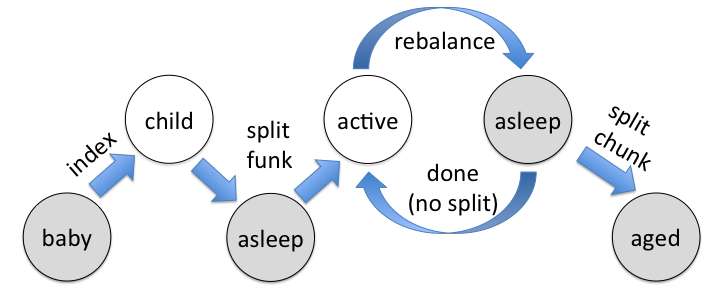
\includegraphics[width=.8\columnwidth]{state-diagram.png}
}
\caption{Chunk life cycle; immutable states are grey and mutable ones are white.
Chunk splits  create new chunks in immutable \emph{baby} state, which changes to the mutable \emph{child} state once they 
are indexed. When the appropriate funks are created, the chunks become \emph{active}. All rebalance operations go through an 
\emph{asleep} state when the chunk is immutable.}
\label{fig:chunklife}
\end{figure}
}

If a munk rebalance exceeds some capacity threshold in a new munk, it triggers a \emph{split}. Unlike 
single-chunk rebalances, splits entail changes in the chunks linked list as well as the index, and so are more subtle. 
A split proceeds in two phases. In the first, the chunk is immutable, namely,  rebalanceLock is held in exclusive mode. In the second (longer) phase, the new chunks are mutable.

The first phase runs in-memory and so is fast (this prevents blocking puts for a long time). 
It proceeds as follows: 
(1) split the munk into two sorted and compacted halves; 
(2) create two new chunks (metadata), each referencing one of the new munks but temporarily sharing the same old funk, both immutable, with the first half munk pointing to the second; 
(3) insert the new chunks into the list instead of the old chunk; and finally  
(4) update the index.
Note that once the new chunks are added to the list they can be discovered by concurrent operations.
On the other hand, other concurrent operations might still access the  old chunk via the index or stale pointers. 
This does not pose a problem because the chunks are immutable and contain the same KV pairs. 

In the second phase, puts are enabled on the new chunks (rebalanceLock is released)
but the new chunks cannot yet be rebalanced. 
Note that the old chunk remains immutable; it continues to serve ongoing reads as long as 
there are outstanding operations that hold references to it, after which it may be  garbage collected.
This phase splits the shared funk. It uses the sorted prefixes of the new munks as SSTables and their 
suffixes as  logs. Once done, the funk references in the new chunks are flipped and future rebalances are allowed.



\remove{
In order to guarantee correctness of this multi-step process, we model a chunk's life cycle as a finite state machine, 
depicted by Figure~\ref{fig:chunklife}. A new chunk is created in \emph{baby} state, in which it is immutable. Once added 
to the index, a chunk transitions to \emph{child} state, in which it is mutable but cannot be rebalanced yet. Finally, when 
a chunk gets its own funk it becomes \emph{active} -- i.e., eligible for all operations. A chunk that has been split into 
two new chunks becomes \emph{aged} -- a state in which it remains immutable but can serve the gets and the scans 
that are concurrently accessing it via the index. Once it gets removed from the chunk list and has no outstanding
reads, it can be disposed. 
%We omit the formal correctness proof for lack of space; see~\cite{kiwi} for similar proofs.   
}

Underflowing neighboring chunks (e.g., following massive deletions) can be merged via a similar protocol. 
Our current \sys\/ prototype does not implement this feature. 
%Merges can be handled the same way by making the two merged munks immutable for the duration of the switch; 
%we do not implement this feature in our prototype.

\subsection{Disk flushes and recovery}
\label{ssec:flush-recovery}

Recall that all puts write to the funk log, regardless of whether the chunk has a munk. 
Funk logs are not replayed on recovery, and so recovery time is not impacted by 
their length.

Like most popular KV-stores, \sys\ supports 
two modes of operation -- \emph{synchronous} and \emph{asynchronous}. In the former,  updates are persisted to disk (using an
\code{fsync} call)
before returning to the user. %, ensuring the written data will survive failures once the operation completes. 
The drawback of this approach is that it is roughly an order-of-magnitude slower than the asynchronous mode.
% in existing KV-stores like RocksDB~\cite{RocksDB} as well as in \sys. 
%In asynchronous mode, updates to funk logs are passed to the OS but might .. 
%are guaranteed to be  persisted only after an explicit \code{fsync} call.  
Asynchronous I/O, where \code{fsync} is only called periodically, 
reduces write latency and increases throughput, but 
may lead to loss of data that was written shortly before a crash. The tradeoffs between the two approaches are 
well known, and the choice is typically left to the user.

\paragraph{Recovery semantics.}
In the synchronous mode, 
%every put operation performs a flush after writing the data in the appropriate funk's \code{log}, and then returns. 
%This ensures that 
the funks always reflect all completed updates. In this case, recovery is straightforward: we simply construct
the chunks linked list and chunk index from the funks on disk, and then the database is immediately ready to serve new requests, populating munks and Bloom filters on-demand.  

In the asynchronous mode, some of the  data written before a crash may be lost, but we  
ensure that the data store consistently reflects a \emph{prefix} of the  values written.
For example, if \code{put(k1, v1)} completes before \code{put(k2, v2)} 
is invoked and then the system crashes, then following the recovery, 
if \code{k2} appears in the data store, then \code{k1} must appear in it as well. 
%conversely, if the update of \code{k1}  is lost, \code{k2}  must be also excluded.
Such recovery to a consistent state is important, since later updates may depend on earlier ones. 

Note that the temporal organization in LSMs inherently guarantees such consistency, whereas with spatial data organization,
extra measures need to be taken to ensure it.

\paragraph{Checkpointing for consistent recovery.}

We use \emph{checkpoints} to support recovery to a consistent state in asynchronous mode.
A background process creates checkpoints using atomic scans: 
It first fetches-and-increments GV to obtain a snapshot version \code{gv}.  Next, 
it synchronizes with pending puts via PO to ensure that all puts with smaller versions are complete. 
It then calls \code{fsync} to flush all pending writes to disk.
Finally, it writes \code{gv} to a dedicated \emph{checkpoint file} on disk.
This enforces the following correctness invariant: at all times, all updates pertaining to versions smaller 
than or equal to the version recorded in the checkpoint file have been persisted.
%indicating that all updates pertaining to versions smaller than or equal to this version have been persisted.
Note that some puts with higher versions than \code{gv} might be reflected on disk while others are not. 

\sys's recovery is lazy. 
%All data is initially on disk, and 
Data is fetched into munks as needed during normal operation. 
To ensure consistency, following a recovery,  
retrievals from funks should ignore newer versions that were not included in the latest completed checkpoint before the crash. 
This must be done by every operation that reads data from a funk, namely get or scan from a chunk without a munk, 
funk rebalance, or munk load. 

To facilitate this check, we distinguish between pre-crash versions and new ones created after recovery using \emph{epoch numbers}. 
Specifically, a version is split into an epoch number (in our implementation, the four most-significant bits of the version) and a per-epoch version number. 
Incrementing the GV in the normal mode effectively increases the latter.
The recovery procedure increments the former and resets the latter, so 
versions in the new epoch begin from zero. 

We maintain a \emph{recoveryTable} mapping each recovered epoch to its last checkpointed version number. 
For example, Table~\ref{table:recovery} shows a possible state of the recovery table after two recoveries, i.e., during epoch $2$. 

\begin{table}
\begin{center}
%\small
\begin{tabular}{ll}
epoch & last checkpointed version \\
\hline
0 & 1375\\
1 &  956\\
\end{tabular}
\end{center}
\caption{Example recovery table during epoch $2$.}
\label{table:recovery}
\end{table} 
 
 \remove{
Every read from a funk  %(during get,  scan, funk rebalance,  or munk load) 
refers to the recovery table in order to identify versions that should be ignored -- 
these are versions from old epochs that exceed the checkpoint number for their epoch. 
}
%\paragraph{Recovery procedure.} 
The recovery procedure reads the checkpoint time from disk, loads the recoveryTable into memory, adds a new row to it with the last epoch and latest checkpoint time, and persists it again. It then increments the epoch number and resumes normal operation with version  $0$ in the new epoch.







